\section{课题计划}
\subsection{课题目的}
通过Logical Regression逻辑回归,SVM支持向量机和LSTM三种方式,对一系列样本数据进行测试,得出每种模型下的结果,并对整体进行分析和改进。
\\\indent{}由于本课题是工程课题,因此本文主要记录了实验过程中的相关信息和数据,并进行分析和改进,涉及到的数理理论分析会比较少
\subsection{课题流程}
\subsubsection{整体流程}
模型建立的整体思路如下: 
\begin{enumerate}
    \item 分别拿到正常请求和恶意请求的数据集。 
    \item 对无规律的数据集进行处理得到特征矩阵。 
    \item 选择某种算法模型,使用特征矩阵训练检测模型。
    \item 最后计算模型的准确度,并使用检测模型判断未知URL 请求是恶意的还是正常的。
\end{enumerate}
本课题中采用了二分类机器学习和序列模式这两种主要方式。
\\\indent{}其中做二分类机器学习的算法有很多,常见的有逻辑回归和svm。本次课题选择这两种分类模型探究识别恶意URL的课题。序列模型的分析话主要是通过使用Keras框架来构建LSTM RNN来对正常或者恶意的网络请求进行区分。
\subsubsection{基于Logical Regression逻辑回归}
Logistic回归是一种广义线性回归(generalized linear model),目的是从特征学习出一个0/1分类模型,而这个模型是将特性的线性组合作为自变量,由于自变量的取值范围是负无穷到正无穷。因此,使用logistic函数(或称作sigmoid函数)将自变量映射到(0,1)上,映射后的值被认为是属于y=1的概率。 
Logistic回归模型的适用条件二分类问题 所以选择逻辑回归做url分类.
\subsubsection{基于SVM支持向量机}
支持向量机(Support Vector Machine,SVM,又名支持向量网络)是在分类与回归分析中分析数据的监督式学习模型与相关的学习算法。给定一组训练实例,每个训练实例被标记为属于两个类别中的一个或另一个,SVM训练算法创建一个将新的实例分配给两个类别之一的模型,使其成为非概率二元线性分类器。SVM模型是将实例表示为空间中的点,这样映射就使得单独类别的实例被尽可能宽的明显的间隔分开。然后,将新的实例映射到同一空间,并基于它们落在间隔的哪一侧来预测所属类别。
\subsubsection{基于LSTM序列模型}
目前很多研究表明,深度学习和神经网络在图像识别和自然语言处理(NLP)方面表现出众。我们可以利用神经网络的NLP能力来处理这个分类问题。
\subsection{课题数据来源}
由于三种测试方法的数据均来自以下,故在第四部分中不再赘述。
对于数据,统一标记为:
\begin{itemize}
    \item 0 =正常请求日志样本
    \item 1 =请求日志表示尝试的注入攻击
\end{itemize}
本项目一共有三大类数据集。\setcounter{footnote}{0}
\footnote{bad-waf.txt,good-waf.txt:来自于Fwaf-Machine-Learning-driven-Web-Application-Firewall项目}
\footnote{bad1.txt, good1.txt,good2.txt:某系统的某天的访问url,已进行清洗去重}
\footnote{dev-access.csv:通过模拟API给出JSON形式的访问请求日志}
% \textbf{negative部分样例:}
\begin{figure}[!h]
    \setlength{\abovecaptionskip}{0.cm}
    \setlength{\belowcaptionskip}{-0.cm}
    \centering
     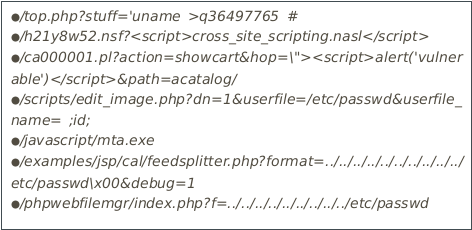
\includegraphics[scale=0.4]{Figs/bad.png}
    \caption{恶意URL部分样例}
    \label{fig:bad_sample}
\end{figure}
% \textbf{postive部分样例:}
\begin{figure}[!h]
    \setlength{\abovecaptionskip}{0.cm}
    \setlength{\belowcaptionskip}{-0.cm}
    \centering
     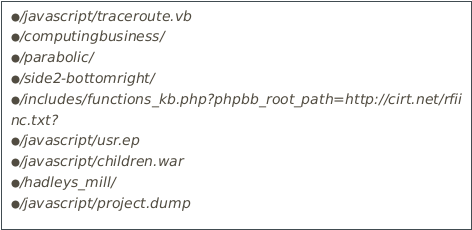
\includegraphics[scale=0.4]{Figs/good.png}
    \caption{正常访问URL部分样例}
    \label{fig:good_sample}
\end{figure}
% \textbf{API模拟json请求数据部分样例:}
\begin{figure}[!h]
    \setlength{\abovecaptionskip}{0.cm}
    \setlength{\belowcaptionskip}{-0.cm}
    \centering
     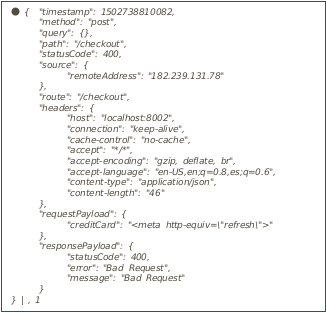
\includegraphics[scale=0.4]{Figs/json.png}
    \caption{API模拟json请求数据部分样例}
    \label{fig:json_sample}
\end{figure}